
%(BEGIN_QUESTION)
% Copyright 2012, Tony R. Kuphaldt, released under the Creative Commons Attribution License (v 1.0)
% This means you may do almost anything with this work of mine, so long as you give me proper credit

In this process, liquefied manure from a dairy farm is mixed with pre-consumer food waste for anaerobic digestion, the purpose of which being to produce ``biogas'' which is largely methane and burns similarly to natural gas.  This biogas is used as fuel for a large engine, which turns a generator to make electricity.  The heated coolant from this engine is piped back to the digester vessel to maintain the organic matter at a temperature similar to the internal temperature of a cow's digestive tract.  Some of the biogas is recycled back into the digester as a means of stirring the liquefied mixture to prevent solids from settling at the bottom and clogging the system:

$$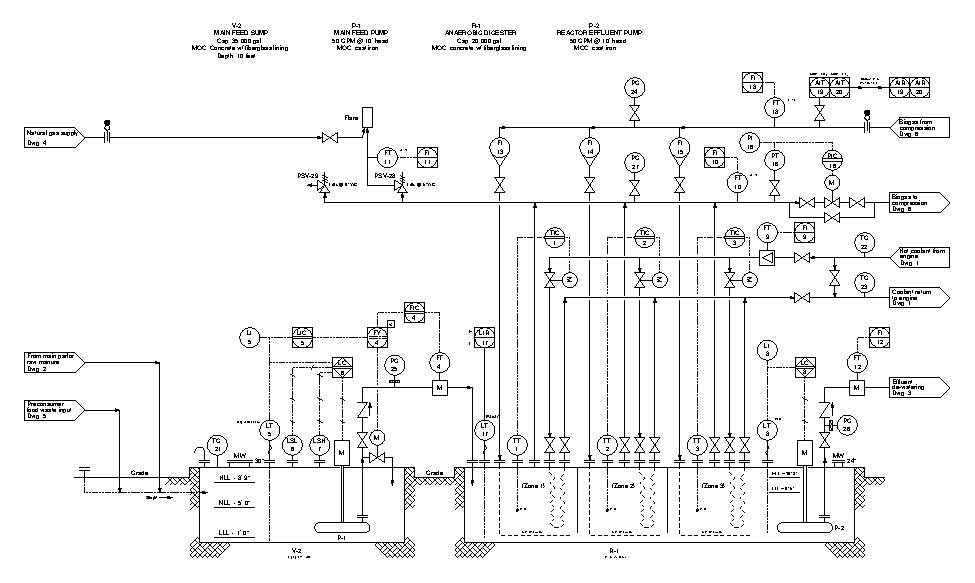
\includegraphics[width=15.5cm]{i0015rx01.eps}$$

Identify the following flowmeter types and comment on why those types are particularly well-suited to the fluid stream they're measuring:

\begin{itemize}
\item{} FT-4 (influent to digester)
\item{} FT-9 (coolant flow from engine)
\item{} FT-10 and FT-18 (biogas flow)
\item{} FT-12 (effluent flow to de-watering)
\end{itemize}

\underbar{file i02146}
%(END_QUESTION)





%(BEGIN_ANSWER)

\begin{itemize}
\item{} {\bf FT-4 (influent to digester):} This is a magnetic flowmeter, which is a good choice for this application because it is non-restrictive, linear, and handles entrained solids with ease.
\vskip 20pt
\item{} {\bf FT-9 (coolant flow from engine):} This is a vortex flowmeter, which is a good choice for this application because it is linear-responding and senses a flow rate that is unlikely to drop below the meter's low-flow cutoff point (because engine coolant flow is critically important and therefore will be at or near full flow at all times).
\vskip 20pt
\item{} {\bf FT-10 and FT-18 (biogas flow):} These are thermal flowmeters, which is a good choice for this application because it is a technology yielding true mass flow rate (ideal for regulatory monitoring, for carbon credits), is linear, and is relatively inexpensive.  The only potential problem in this application is the potential of the biogas composition to change with changes in biomass chemistry.  Thermal mass flowmeters are dependent upon the fluid's specific heat value remaining constant (or at least known), and in this case changes in biogas composition may effect specific heat and therefore introduce errors.
\vskip 20pt
\item{} {\bf FT-12 (effluent flow to de-watering):} This is another magnetic flowmeter, which is a good choice for this application because it is non-restrictive, linear, and handles entrained solids with ease.
\end{itemize}

%(END_ANSWER)





%(BEGIN_NOTES)


%INDEX% Process: anaerobic digester (realistic P&ID shown)

%(END_NOTES)


